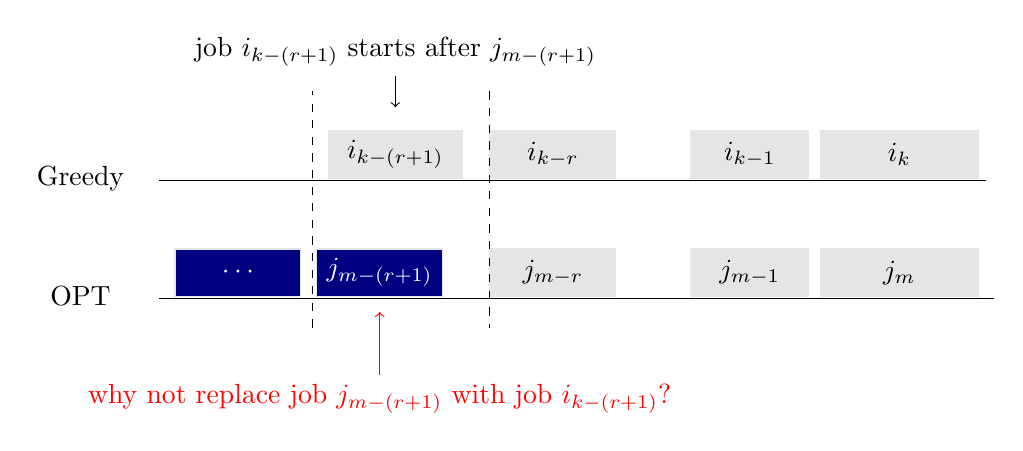
\begin{tikzpicture}
\tikzstyle{timeblock}=[minimum height = 0.6cm,draw=gray!20,fill=gray!20];

\draw (5.5,1.47) -> (-5,1.47);
\draw (5.6,-0.03) -> (-5,-0.03);
\node at (-6,1.5) {Greedy};
\node at (-6,0) {OPT};
\node [timeblock,minimum width=2cm] at (4.4,1.8) {$i_k$};
\node [timeblock,minimum width=2cm] at (4.4,0.3) {$j_m$};
\node [timeblock,minimum width=1.5cm] at (2.5,1.8) {$i_{k-1}$};
\node [timeblock,minimum width=1.5cm] at (2.5,0.3) {$j_{m-1}$};
\node [timeblock,minimum width=1.6cm] at (0,1.8) {$i_{k-r}$};
\node [timeblock,minimum width=1.6cm] at (0,0.3) {$j_{m-r}$};
\draw[dashed] (-0.8,2.6) -- (-0.8,-0.4);
\node [timeblock,minimum width=1.7cm] at (-2,1.8) {$i_{k-(r+1)}$};
\node [timeblock,minimum width=1.6cm,fill=blue!50!black,text=white] at (-2.2,0.3) {$j_{m-(r+1)}$};
\node [timeblock,minimum width=1.6cm,fill=blue!50!black,text=white] at (-4,0.3) {$\cdots$};
\draw[dashed] (-3.05,-0.4) -- (-3.05,2.6);
\draw[->] node [above] at (-2,2.8) {job $i_{k-(r+1)}$ starts after $j_{m-(r+1)}$} edge (-2,2.4);
\draw[->,red] node [below] at (-2.2,-1) {why not replace job $j_{m-(r+1)}$ with job $i_{k-(r+1)}$?} edge (-2.2,-0.2);
\end{tikzpicture}
